\documentclass{article}
\usepackage[paperwidth=18cm,paperheight=13cm,margin=0.45cm]{geometry}
\usepackage{tikz}
\usepackage{xcolor}
\pagestyle{empty}
\definecolor{trainblue}{RGB}{31,119,180}
\definecolor{valred}{RGB}{214,39,40}
\definecolor{gengreen}{RGB}{44,160,44}
\definecolor{discpurple}{RGB}{148,103,189}
\begin{document}
\noindent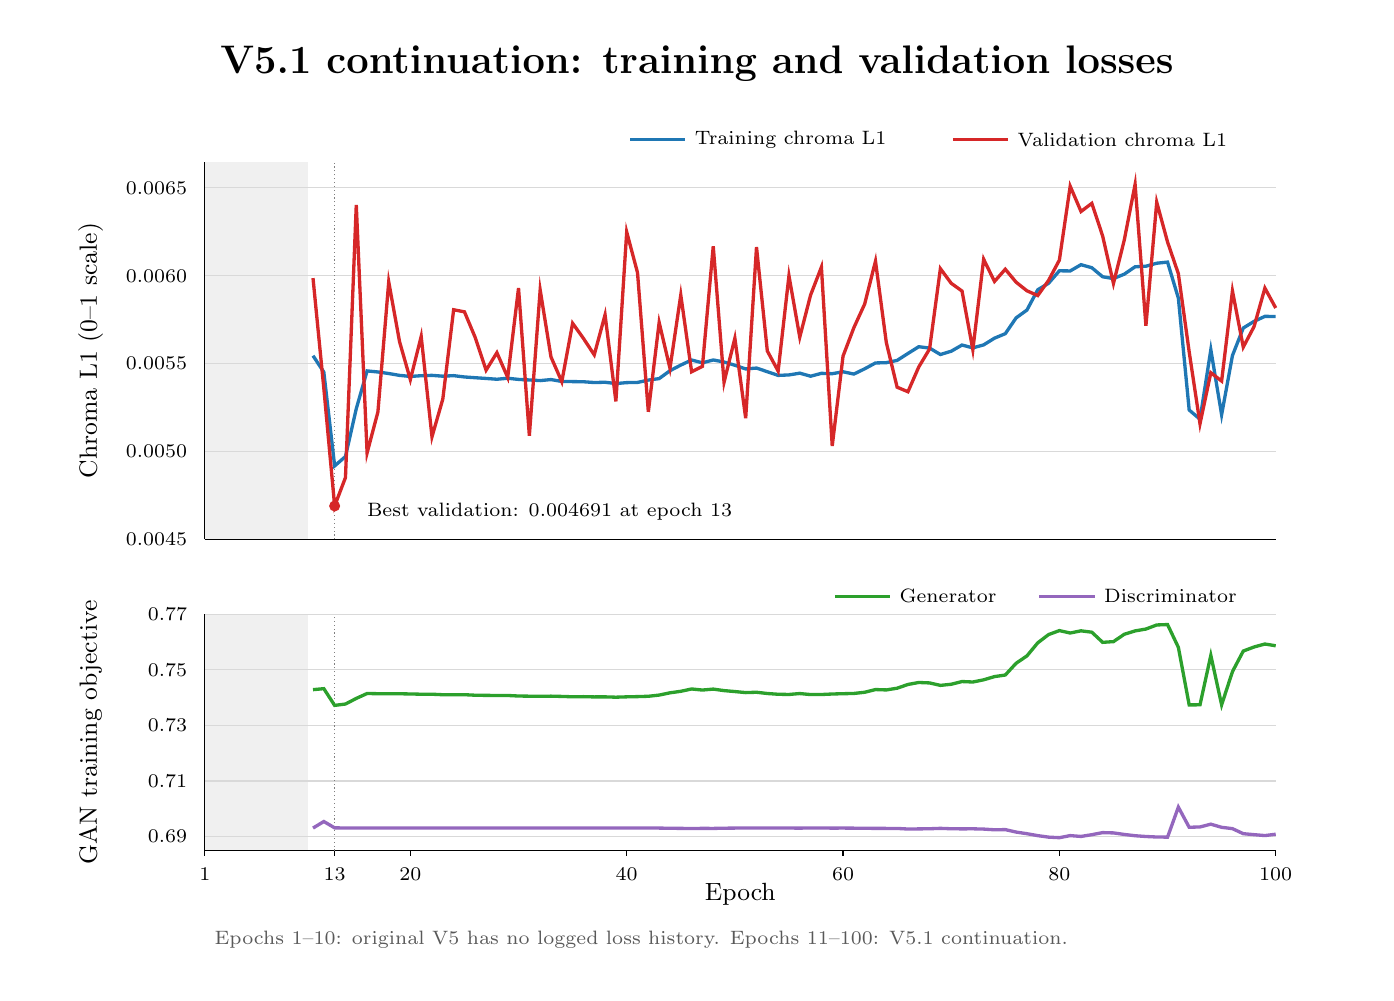
\begin{tikzpicture}[x=1cm,y=1cm]
\path[use as bounding box] (0,0) rectangle (17,12);
\node[font=\Large\bfseries] at (8.5,11.55) {V5.1 continuation: training and validation losses};
\begin{scope}[shift={(2.25,5.5)}]
\fill[gray!12] (0,0) rectangle (1.3051,4.8);
\draw[gray!30,thin] (0,0.0000) -- (13.6, 0.0000);
\node[anchor=east,font=\scriptsize] at (-0.10,0.0000) {0.0045};
\draw[gray!30,thin] (0,1.1163) -- (13.6, 1.1163);
\node[anchor=east,font=\scriptsize] at (-0.10,1.1163) {0.0050};
\draw[gray!30,thin] (0,2.2326) -- (13.6, 2.2326);
\node[anchor=east,font=\scriptsize] at (-0.10,2.2326) {0.0055};
\draw[gray!30,thin] (0,3.3488) -- (13.6, 3.3488);
\node[anchor=east,font=\scriptsize] at (-0.10,3.3488) {0.0060};
\draw[gray!30,thin] (0,4.4651) -- (13.6, 4.4651);
\node[anchor=east,font=\scriptsize] at (-0.10,4.4651) {0.0065};
\draw[black,thin] (0,0) -- (13.6,0);
\draw[black,thin] (0,0) -- (0,4.8);
\draw[gray,densely dotted] (1.6485,0) -- (1.6485,4.8);
\draw[trainblue,very thick] plot coordinates {(1.3737,2.3339) (1.5111,2.1256) (1.6485,0.9342) (1.7859,1.0535) (1.9232,1.6608) (2.0606,2.1407) (2.1980,2.1273) (2.3354,2.1075) (2.4727,2.0841) (2.6101,2.0705) (2.7475,2.0799) (2.8848,2.0843) (3.0222,2.0738) (3.1596,2.0806) (3.2970,2.0639) (3.4343,2.0543) (3.5717,2.0451) (3.7091,2.0349) (3.8465,2.0477) (3.9838,2.0328) (4.1212,2.0259) (4.2586,2.0178) (4.3960,2.0308) (4.5333,2.0071) (4.6707,2.0051) (4.8081,2.0031) (4.9455,1.9931) (5.0828,1.9968) (5.2202,1.9799) (5.3576,1.9922) (5.4949,1.9945) (5.6323,2.0243) (5.7697,2.0431) (5.9071,2.1434) (6.0444,2.2149) (6.1818,2.2794) (6.3192,2.2432) (6.4566,2.2798) (6.5939,2.2540) (6.7313,2.2126) (6.8687,2.1659) (7.0061,2.1769) (7.1434,2.1308) (7.2808,2.0838) (7.4182,2.0897) (7.5556,2.1122) (7.6929,2.0735) (7.8303,2.1098) (7.9677,2.1055) (8.1051,2.1297) (8.2424,2.1008) (8.3798,2.1675) (8.5172,2.2419) (8.6545,2.2453) (8.7919,2.2743) (8.9293,2.3622) (9.0667,2.4479) (9.2040,2.4309) (9.3414,2.3491) (9.4788,2.3909) (9.6162,2.4695) (9.7535,2.4332) (9.8909,2.4715) (10.0283,2.5564) (10.1657,2.6137) (10.3030,2.8142) (10.4404,2.9136) (10.5778,3.1711) (10.7152,3.2538) (10.8525,3.4122) (10.9899,3.4104) (11.1273,3.4899) (11.2646,3.4511) (11.4020,3.3365) (11.5394,3.3130) (11.6768,3.3695) (11.8141,3.4633) (11.9515,3.4701) (12.0889,3.5085) (12.2263,3.5227) (12.3636,3.0654) (12.5010,1.6444) (12.6384,1.5270) (12.7758,2.4093) (12.9131,1.5845) (13.0505,2.3360) (13.1879,2.6854) (13.3253,2.7701) (13.4626,2.8336) (13.6000,2.8317)};
\draw[valred,very thick] plot coordinates {(1.3737,3.3193) (1.5111,1.9192) (1.6485,0.4254) (1.7859,0.7865) (1.9232,4.2483) (2.0606,1.0995) (2.1980,1.6201) (2.3354,3.2713) (2.4727,2.5127) (2.6101,2.0294) (2.7475,2.5795) (2.8848,1.3044) (3.0222,1.7836) (3.1596,2.9174) (3.2970,2.8911) (3.4343,2.5637) (3.5717,2.1498) (3.7091,2.3721) (3.8465,2.0578) (3.9838,3.1921) (4.1212,1.3187) (4.2586,3.1698) (4.3960,2.3181) (4.5333,2.0038) (4.6707,2.7457) (4.8081,2.5538) (4.9455,2.3448) (5.0828,2.8534) (5.2202,1.7541) (5.3576,3.9051) (5.4949,3.3888) (5.6323,1.6212) (5.7697,2.7560) (5.9071,2.1736) (6.0444,3.1047) (6.1818,2.1302) (6.3192,2.1988) (6.4566,3.7236) (6.5939,1.9965) (6.7313,2.5561) (6.8687,1.5406) (7.0061,3.7129) (7.1434,2.3939) (7.2808,2.1387) (7.4182,3.3495) (7.5556,2.5694) (7.6929,3.1038) (7.8303,3.4589) (7.9677,1.1880) (8.1051,2.3290) (8.2424,2.6895) (8.3798,2.9902) (8.5172,3.5347) (8.6545,2.5020) (8.7919,1.9341) (8.9293,1.8762) (9.0667,2.1907) (9.2040,2.4196) (9.3414,3.4395) (9.4788,3.2537) (9.6162,3.1549) (9.7535,2.4107) (9.8909,3.5588) (10.0283,3.2769) (10.1657,3.4323) (10.3030,3.2672) (10.4404,3.1583) (10.5778,3.0979) (10.7152,3.2901) (10.8525,3.5483) (10.9899,4.4865) (11.1273,4.1655) (11.2646,4.2688) (11.4020,3.8545) (11.5394,3.2517) (11.6768,3.8037) (11.8141,4.5098) (11.9515,2.7139) (12.0889,4.2831) (12.2263,3.7780) (12.3636,3.3752) (12.5010,2.3832) (12.6384,1.4696) (12.7758,2.1179) (12.9131,2.0120) (13.0505,3.1563) (13.1879,2.4434) (13.3253,2.7047) (13.4626,3.1924) (13.6000,2.9398)};
\fill[valred] (1.6485,0.4254) circle (2pt);
\node[anchor=west,font=\scriptsize,fill=white,inner sep=1.5pt] at (2.0,0.35) {Best validation: 0.004691 at epoch 13};
\node[rotate=90,font=\small] at (-1.45,2.4) {Chroma L1 (0--1 scale)};
\draw[trainblue,very thick] (5.4,5.08) -- (6.1,5.08);
\node[anchor=west,font=\scriptsize,fill=white,inner sep=1pt] at (6.18,5.08) {Training chroma L1};
\draw[valred,very thick] (9.5,5.08) -- (10.2,5.08);
\node[anchor=west,font=\scriptsize,fill=white,inner sep=1pt] at (10.28,5.08) {Validation chroma L1};
\end{scope}
\begin{scope}[shift={(2.25,1.55)}]
\fill[gray!12] (0,0) rectangle (1.3051,3.0);
\draw[gray!30,thin] (0,0.1765) -- (13.6,0.1765);
\node[anchor=east,font=\scriptsize] at (-0.10,0.1765) {0.69};
\draw[gray!30,thin] (0,0.8824) -- (13.6,0.8824);
\node[anchor=east,font=\scriptsize] at (-0.10,0.8824) {0.71};
\draw[gray!30,thin] (0,1.5882) -- (13.6,1.5882);
\node[anchor=east,font=\scriptsize] at (-0.10,1.5882) {0.73};
\draw[gray!30,thin] (0,2.2941) -- (13.6,2.2941);
\node[anchor=east,font=\scriptsize] at (-0.10,2.2941) {0.75};
\draw[gray!30,thin] (0,3.0000) -- (13.6,3.0000);
\node[anchor=east,font=\scriptsize] at (-0.10,3.0000) {0.77};
\draw[black,thin] (0,0) -- (13.6,0);
\draw[black,thin] (0,0) -- (0,3.0);
\draw[gray,densely dotted] (1.6485,0) -- (1.6485,3.0);
\draw[gengreen,very thick] plot coordinates {(1.3737,2.0426) (1.5111,2.0554) (1.6485,1.8428) (1.7859,1.8602) (1.9232,1.9316) (2.0606,1.9939) (2.1980,1.9915) (2.3354,1.9919) (2.4727,1.9906) (2.6101,1.9880) (2.7475,1.9848) (2.8848,1.9848) (3.0222,1.9784) (3.1596,1.9778) (3.2970,1.9788) (3.4343,1.9720) (3.5717,1.9700) (3.7091,1.9692) (3.8465,1.9688) (3.9838,1.9619) (4.1212,1.9599) (4.2586,1.9581) (4.3960,1.9603) (4.5333,1.9568) (4.6707,1.9523) (4.8081,1.9539) (4.9455,1.9506) (5.0828,1.9513) (5.2202,1.9470) (5.3576,1.9515) (5.4949,1.9544) (5.6323,1.9587) (5.7697,1.9739) (5.9071,2.0026) (6.0444,2.0219) (6.1818,2.0514) (6.3192,2.0378) (6.4566,2.0499) (6.5939,2.0307) (6.7313,2.0186) (6.8687,2.0054) (7.0061,2.0098) (7.1434,1.9939) (7.2808,1.9842) (7.4182,1.9817) (7.5556,1.9933) (7.6929,1.9805) (7.8303,1.9811) (7.9677,1.9875) (8.1051,1.9914) (8.2424,1.9945) (8.3798,2.0096) (8.5172,2.0441) (8.6545,2.0393) (8.7919,2.0611) (8.9293,2.1087) (9.0667,2.1339) (9.2040,2.1282) (9.3414,2.0971) (9.4788,2.1112) (9.6162,2.1459) (9.7535,2.1398) (9.8909,2.1678) (10.0283,2.2085) (10.1657,2.2286) (10.3030,2.3779) (10.4404,2.4713) (10.5778,2.6374) (10.7152,2.7422) (10.8525,2.7929) (10.9899,2.7621) (11.1273,2.7899) (11.2646,2.7724) (11.4020,2.6437) (11.5394,2.6528) (11.6768,2.7461) (11.8141,2.7888) (11.9515,2.8125) (12.0889,2.8644) (12.2263,2.8695) (12.3636,2.5805) (12.5010,1.8494) (12.6384,1.8502) (12.7758,2.4782) (12.9131,1.8502) (13.0505,2.2717) (13.1879,2.5330) (13.3253,2.5849) (13.4626,2.6224) (13.6000,2.6001)};
\draw[discpurple,very thick] plot coordinates {(1.3737,0.2849) (1.5111,0.3682) (1.6485,0.2877) (1.7859,0.2861) (1.9232,0.2866) (2.0606,0.2857) (2.1980,0.2856) (2.3354,0.2853) (2.4727,0.2851) (2.6101,0.2850) (2.7475,0.2853) (2.8848,0.2854) (3.0222,0.2853) (3.1596,0.2850) (3.2970,0.2852) (3.4343,0.2853) (3.5717,0.2854) (3.7091,0.2853) (3.8465,0.2853) (3.9838,0.2852) (4.1212,0.2852) (4.2586,0.2852) (4.3960,0.2852) (4.5333,0.2853) (4.6707,0.2853) (4.8081,0.2854) (4.9455,0.2856) (5.0828,0.2853) (5.2202,0.2856) (5.3576,0.2854) (5.4949,0.2854) (5.6323,0.2850) (5.7697,0.2847) (5.9071,0.2823) (6.0444,0.2810) (6.1818,0.2793) (6.3192,0.2810) (6.4566,0.2804) (6.5939,0.2833) (6.7313,0.2847) (6.8687,0.2858) (7.0061,0.2859) (7.1434,0.2859) (7.2808,0.2860) (7.4182,0.2854) (7.5556,0.2840) (7.6929,0.2867) (7.8303,0.2857) (7.9677,0.2844) (8.1051,0.2849) (8.2424,0.2838) (8.3798,0.2822) (8.5172,0.2811) (8.6545,0.2806) (8.7919,0.2803) (8.9293,0.2728) (9.0667,0.2745) (9.2040,0.2763) (9.3414,0.2815) (9.4788,0.2762) (9.6162,0.2748) (9.7535,0.2756) (9.8909,0.2720) (10.0283,0.2631) (10.1657,0.2654) (10.3030,0.2341) (10.4404,0.2134) (10.5778,0.1890) (10.7152,0.1699) (10.8525,0.1627) (10.9899,0.1893) (11.1273,0.1786) (11.2646,0.2009) (11.4020,0.2272) (11.5394,0.2234) (11.6768,0.2039) (11.8141,0.1877) (11.9515,0.1779) (12.0889,0.1714) (12.2263,0.1698) (12.3636,0.5509) (12.5010,0.2950) (12.6384,0.2992) (12.7758,0.3344) (12.9131,0.2945) (13.0505,0.2775) (13.1879,0.2137) (13.3253,0.2011) (13.4626,0.1898) (13.6000,0.2066)};
\node[rotate=90,font=\small] at (-1.45,1.5) {GAN training objective};
\draw[gengreen,very thick] (8.0,3.23) -- (8.7,3.23);
\node[anchor=west,font=\scriptsize,fill=white,inner sep=1pt] at (8.78,3.23) {Generator};
\draw[discpurple,very thick] (10.6,3.23) -- (11.3,3.23);
\node[anchor=west,font=\scriptsize,fill=white,inner sep=1pt] at (11.38,3.23) {Discriminator};
\draw (0.0000,0) -- (0.0000,-0.07);
\node[anchor=north,font=\scriptsize] at (0.0000,-0.10) {1};
\draw (1.6485,0) -- (1.6485,-0.07);
\node[anchor=north,font=\scriptsize] at (1.6485,-0.10) {13};
\draw (2.6101,0) -- (2.6101,-0.07);
\node[anchor=north,font=\scriptsize] at (2.6101,-0.10) {20};
\draw (5.3576,0) -- (5.3576,-0.07);
\node[anchor=north,font=\scriptsize] at (5.3576,-0.10) {40};
\draw (8.1051,0) -- (8.1051,-0.07);
\node[anchor=north,font=\scriptsize] at (8.1051,-0.10) {60};
\draw (10.8525,0) -- (10.8525,-0.07);
\node[anchor=north,font=\scriptsize] at (10.8525,-0.10) {80};
\draw (13.6000,0) -- (13.6000,-0.07);
\node[anchor=north,font=\scriptsize] at (13.6000,-0.10) {100};
\node[font=\small] at (6.8,-0.56) {Epoch};
\end{scope}
\node[anchor=west,font=\scriptsize,text=gray!70!black] at (2.25,0.42) {Epochs 1--10: original V5 has no logged loss history. Epochs 11--100: V5.1 continuation.};
\end{tikzpicture}
\end{document}
